\documentclass{beamer}
\usepackage{subfig}
\usepackage{amsmath}
\usepackage{bm}

\DeclareMathOperator*{\argmax}{arg\,max}
\DeclareMathOperator*{\argmin}{arg\,min}


\title{Logistic Regression}
\author{Prof. Alessandro Lucantonio}
\institute{Aarhus University - Department of Mechanical and Production Engineering}
\date{?/?/2023}

\begin{document}
	\frame{\titlepage}
	
	\begin{frame}
		\frametitle{Binary classification}
		Classification : discrete target (output vector).
		
		Binary classification: $\{0,1\}$ target
		
		\vspace{5mm}
		Example of binary classification task: Spam/not spam emails.
		
		\vspace{5mm}
		Idea: consider hypothesis $h_w$ such that
		\begin{equation*}
			0 \leq h_{\bm{w}} \leq 1.
		\end{equation*}

		\begin{itemize}
			\item if $h_{\bm{w}}(\bm{x}) \geq 0.5$, predict $1$;
			\item if $h_{\bm{w}}(\bm{x}) < 0.5$, predict $0$.
		\end{itemize}
	\end{frame}

	\begin{frame}
		\frametitle{Logistic Regression}
		Hypothesis: $h_{\bm{w}}(\bm{x}) = \sigma(\bm{w}^T\bm{x})$, where
		\begin{equation*}
			\sigma(t) = \frac{1}{1+e^{-t}}
		\end{equation*}
		is the \textbf{sigmoid function}.
		
		\begin{figure}
			\centering
			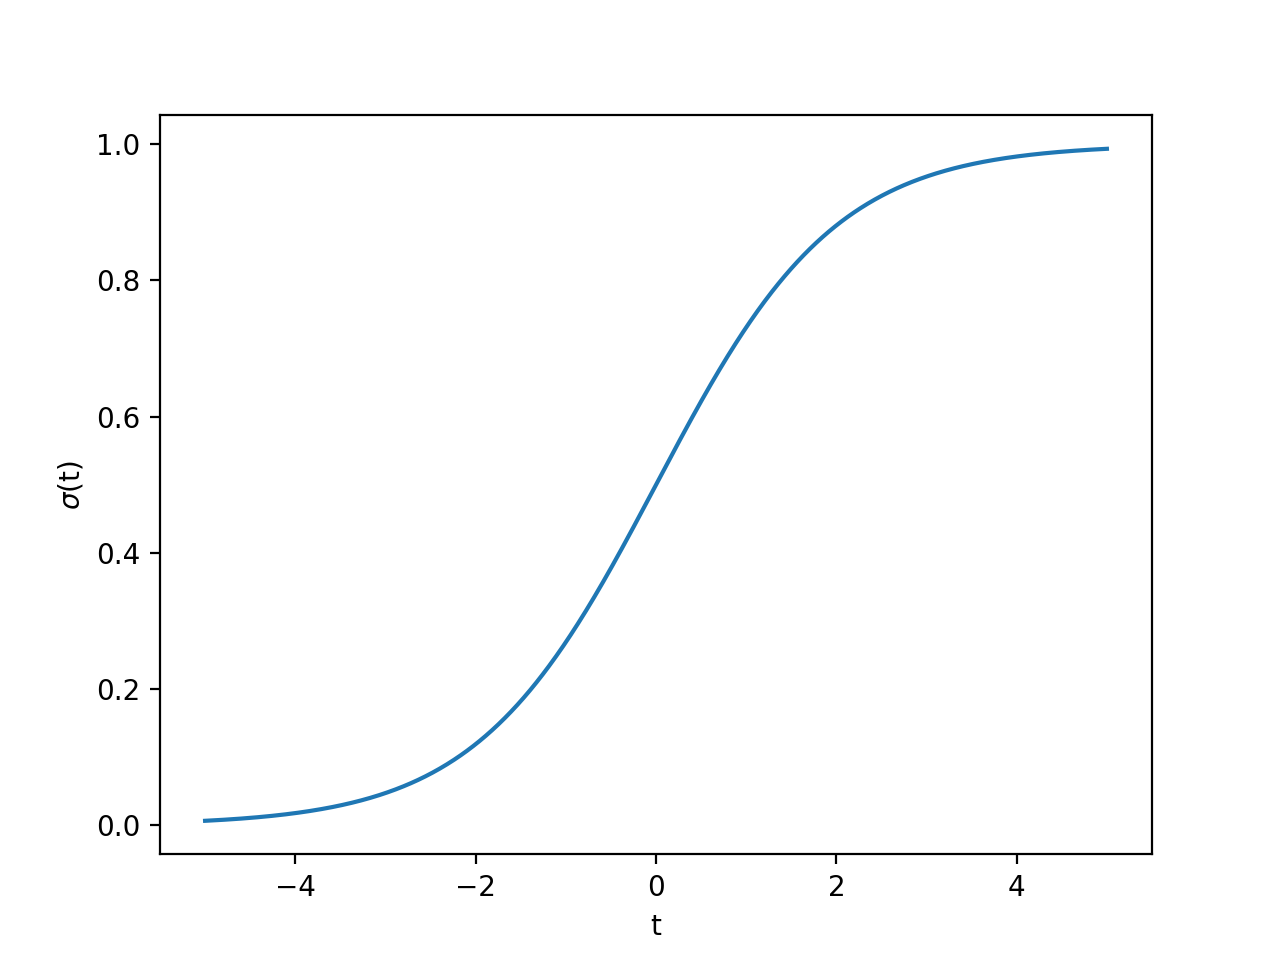
\includegraphics[scale=0.45]{images/sigmoid}
			\caption{Sigmoid function}
		\end{figure}
		
	\end{frame}

	\begin{frame}
		\frametitle{Linear decision boundary}
		Model: $h_{\bm{w}}(x_1, x_2) = \sigma(w_0 + w_1 x_1 + w_2 x_2)$
		\begin{figure}
			\centering
			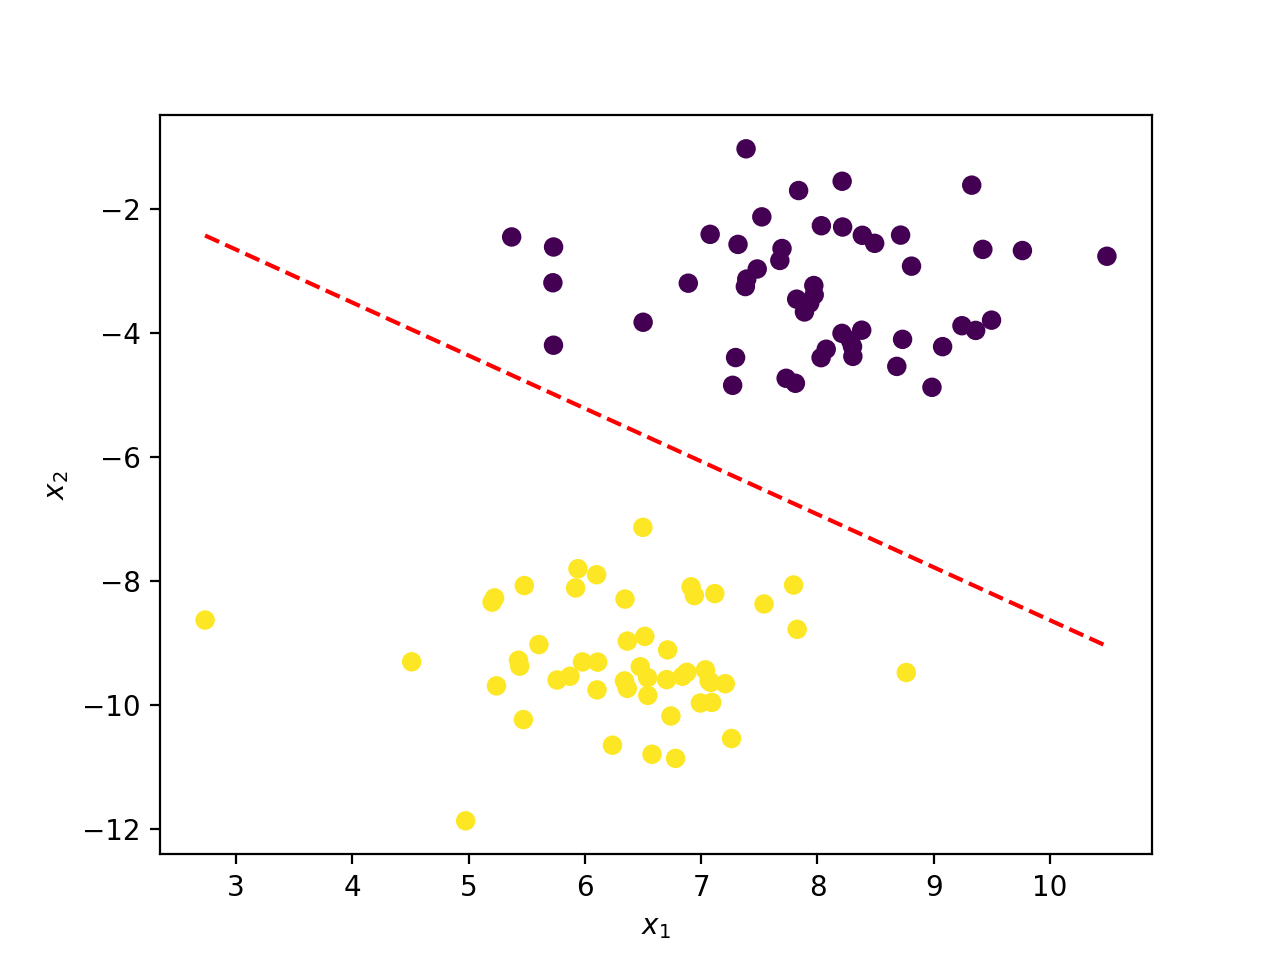
\includegraphics[scale=0.5]{images/linear_decision_boundary}
			\caption{An example of linear decision boundary}
		\end{figure}
	\end{frame}

	\begin{frame}
		\frametitle{Non-linear decision boundary}
		Model: $h_{\bm{w}}(x_1, x_2) = \sigma(w_0 + w_1 x_1 + w_2 x_2 + w_3 x_1^2 + w_4 x_2^2)$
		\begin{figure}
			\centering
			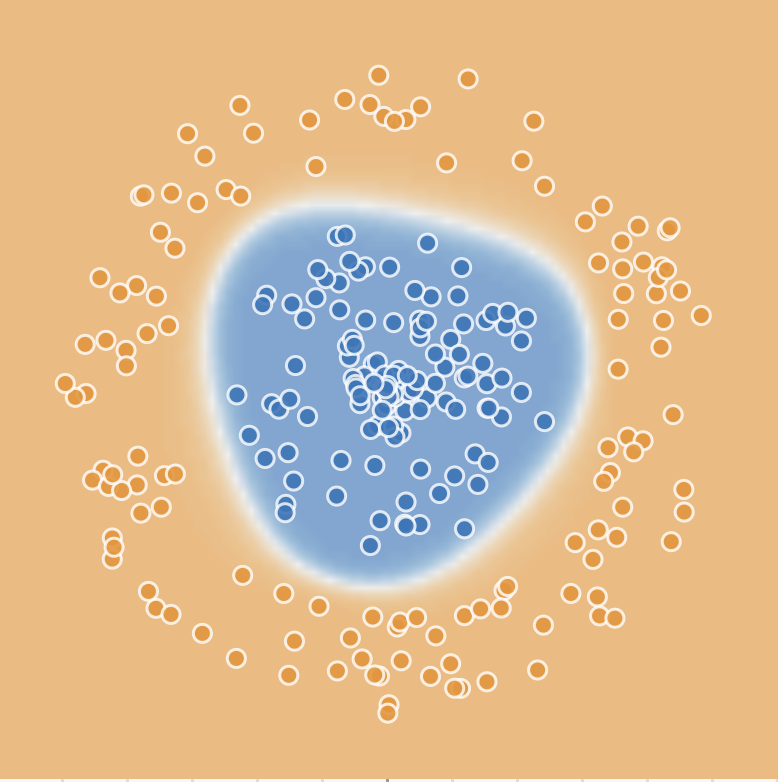
\includegraphics[scale=0.8]{images/non-linear-decision-boundary}
			\caption{An example of non-linear decision boundary}
		\end{figure}
	\end{frame}

	\begin{frame}
		\frametitle{Cost function}
		
		First try: MSE
		\begin{equation*}
			E(\bm{w}) = \frac{1}{N} \sum_{i= 0}^{N} (\sigma(\bm{w}^T\bm{x^i}) - y)^2
		\end{equation*}
		
		Huge problem: $\sigma$ \textsl{non-convex}, hence MSE is \textsl{non-convex} (many local minima).
		
		\vspace{5mm}
		
		Main idea: if $y=1$ the prediction $h_{\bm{w}}(x)$ is good when $h_{\bm{w}}(x) \approx 1$. Good prediction means low error and $\log(1) = 0$.
		
		\vspace{5mm}
		
		Second try: \textbf{Binary cross-entropy}
		\begin{equation*}
			E(\bm{w}) := - \frac{1}{N} \sum_{i=1}^{N} y^i\log(h_{\bm{w}}(x^i)) + (1-y^i)\log(1-h_{\bm{w}}(x^i))
		\end{equation*}
		
		
		
	\end{frame}

	\begin{frame}
		\frametitle{Parenthesis - What is a convex function?}
		A function is \textsl{convex} when for all pairs of points on the graph, the line segment that connects these two points passes above the curve.
		
		A function is \textsl{concave} when its opposite is convex.
		
		\begin{figure}
			\centering
			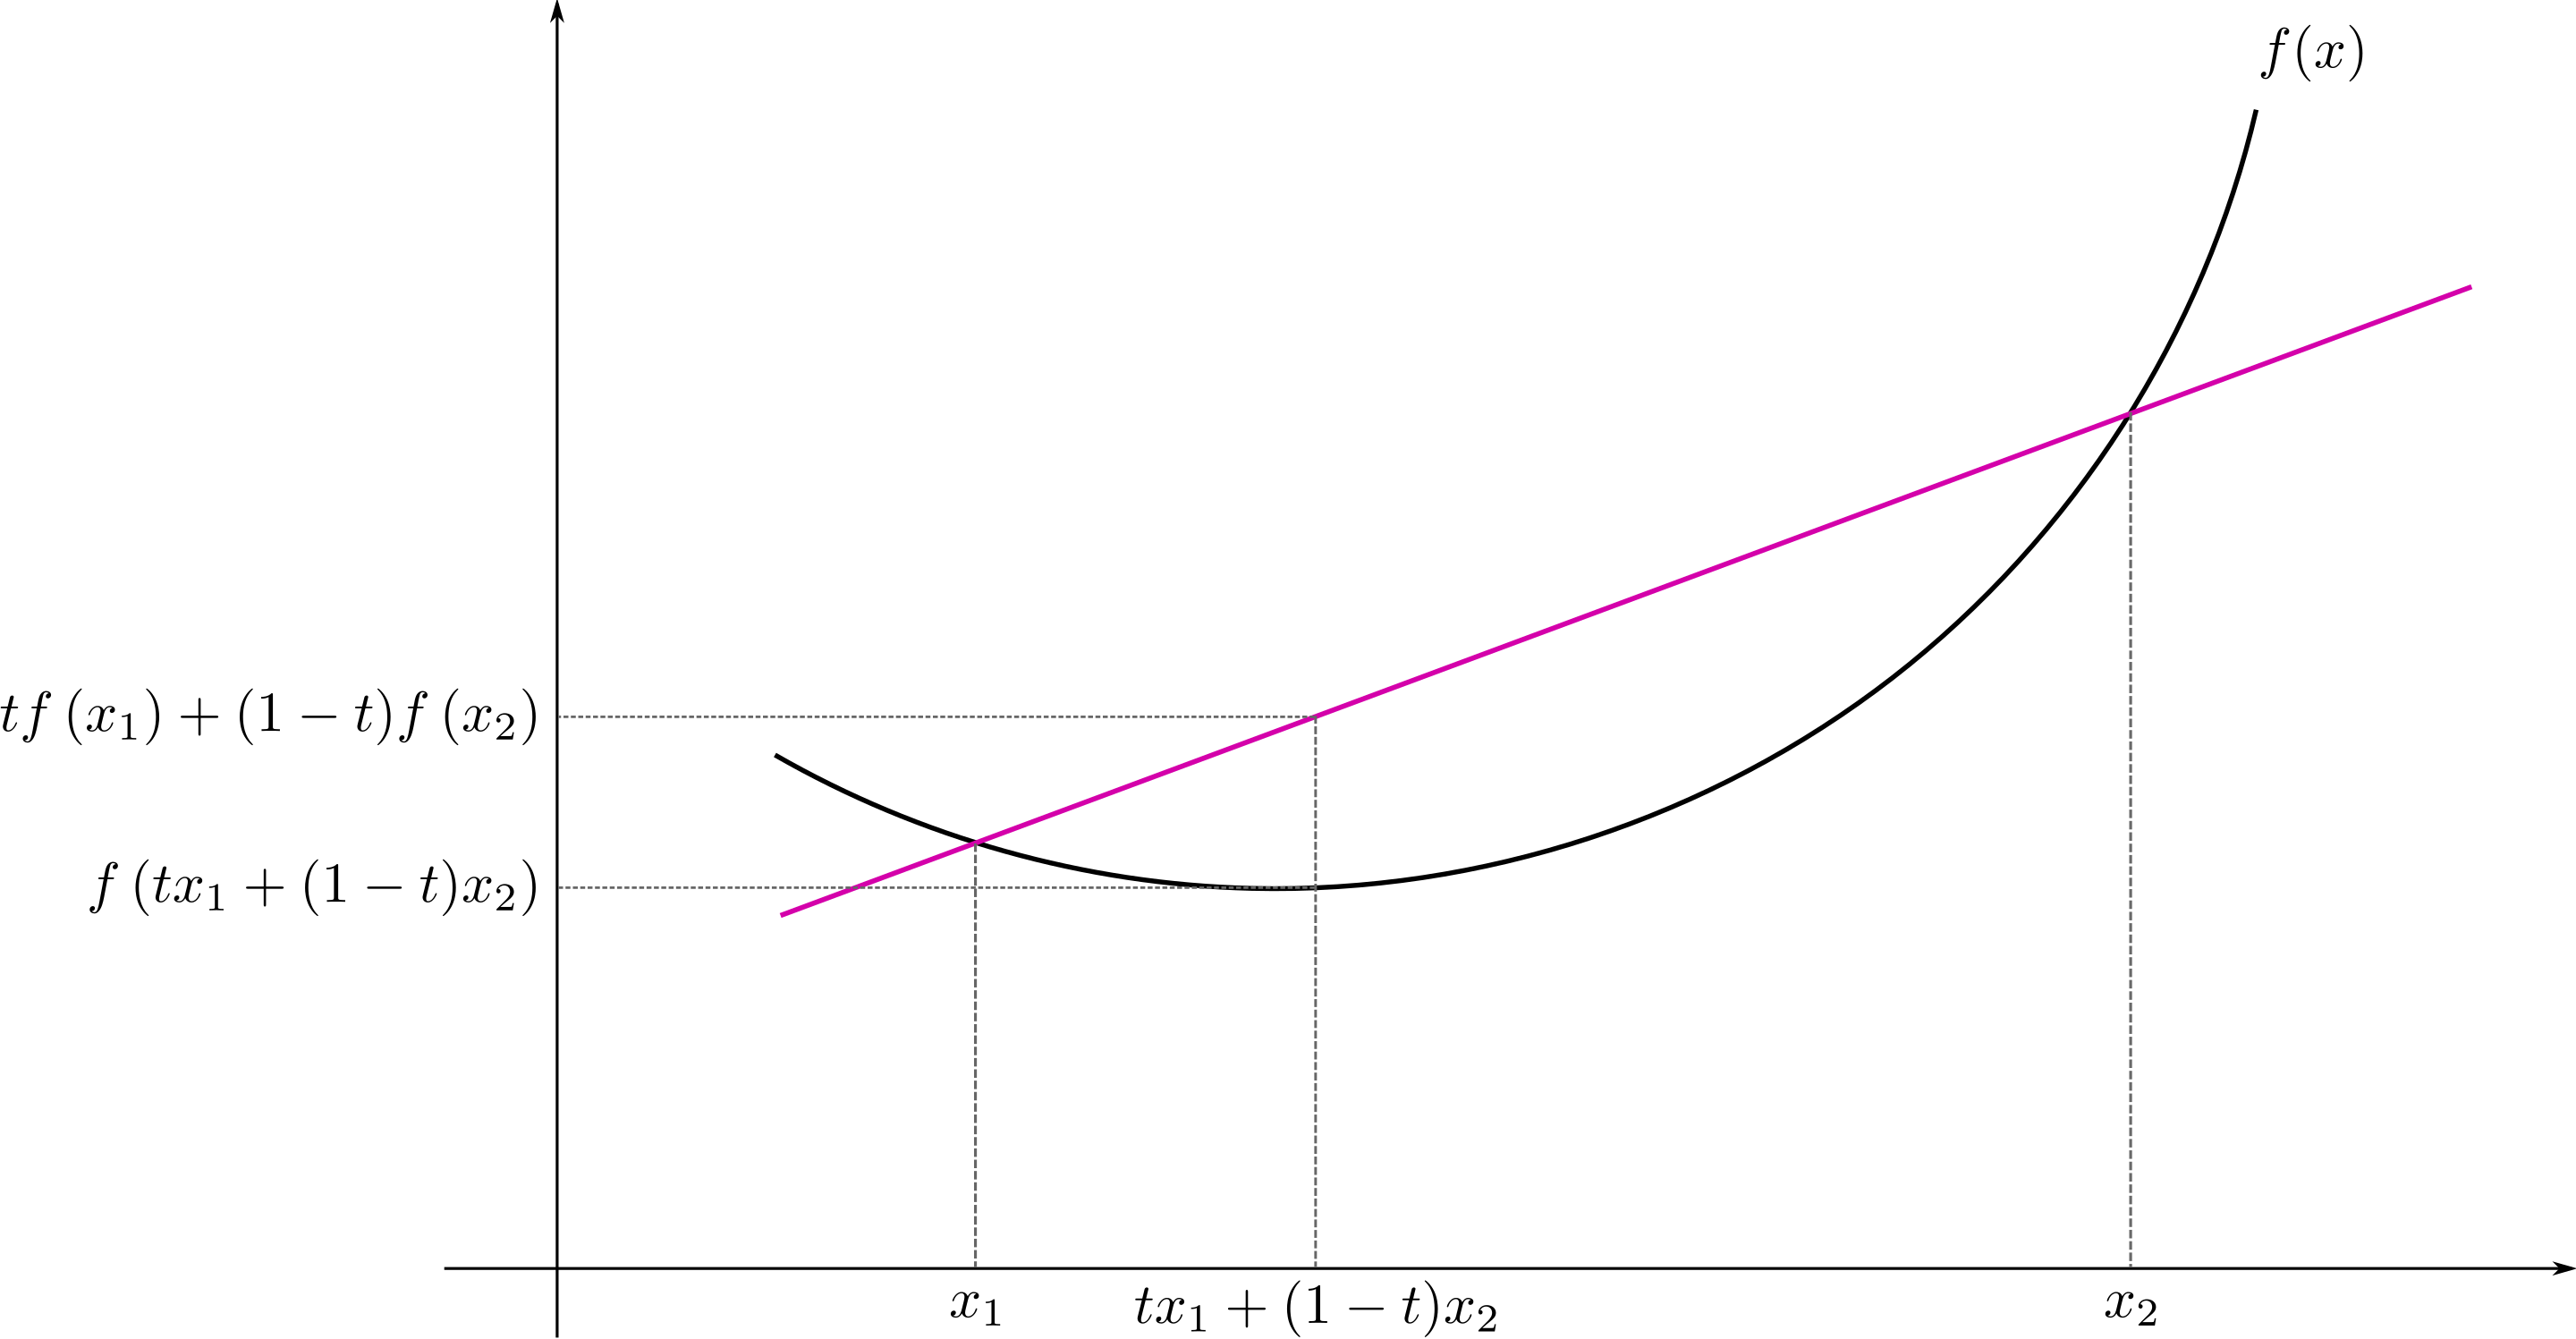
\includegraphics[scale=0.1]{images/convexity}
			\caption{Geometric intuition of convexity}
		\end{figure}
	\end{frame}

	\begin{frame}
		\frametitle{Parenthesis - The power of convexity}
		Any local minimum of a convex function is also a global minimum. 
		Instead, a non-convex function has potentially many local minima which are not global minima and many saddle points (points with null gradient but nor minimum nor maximum).
		
		\begin{figure}
			\centering
			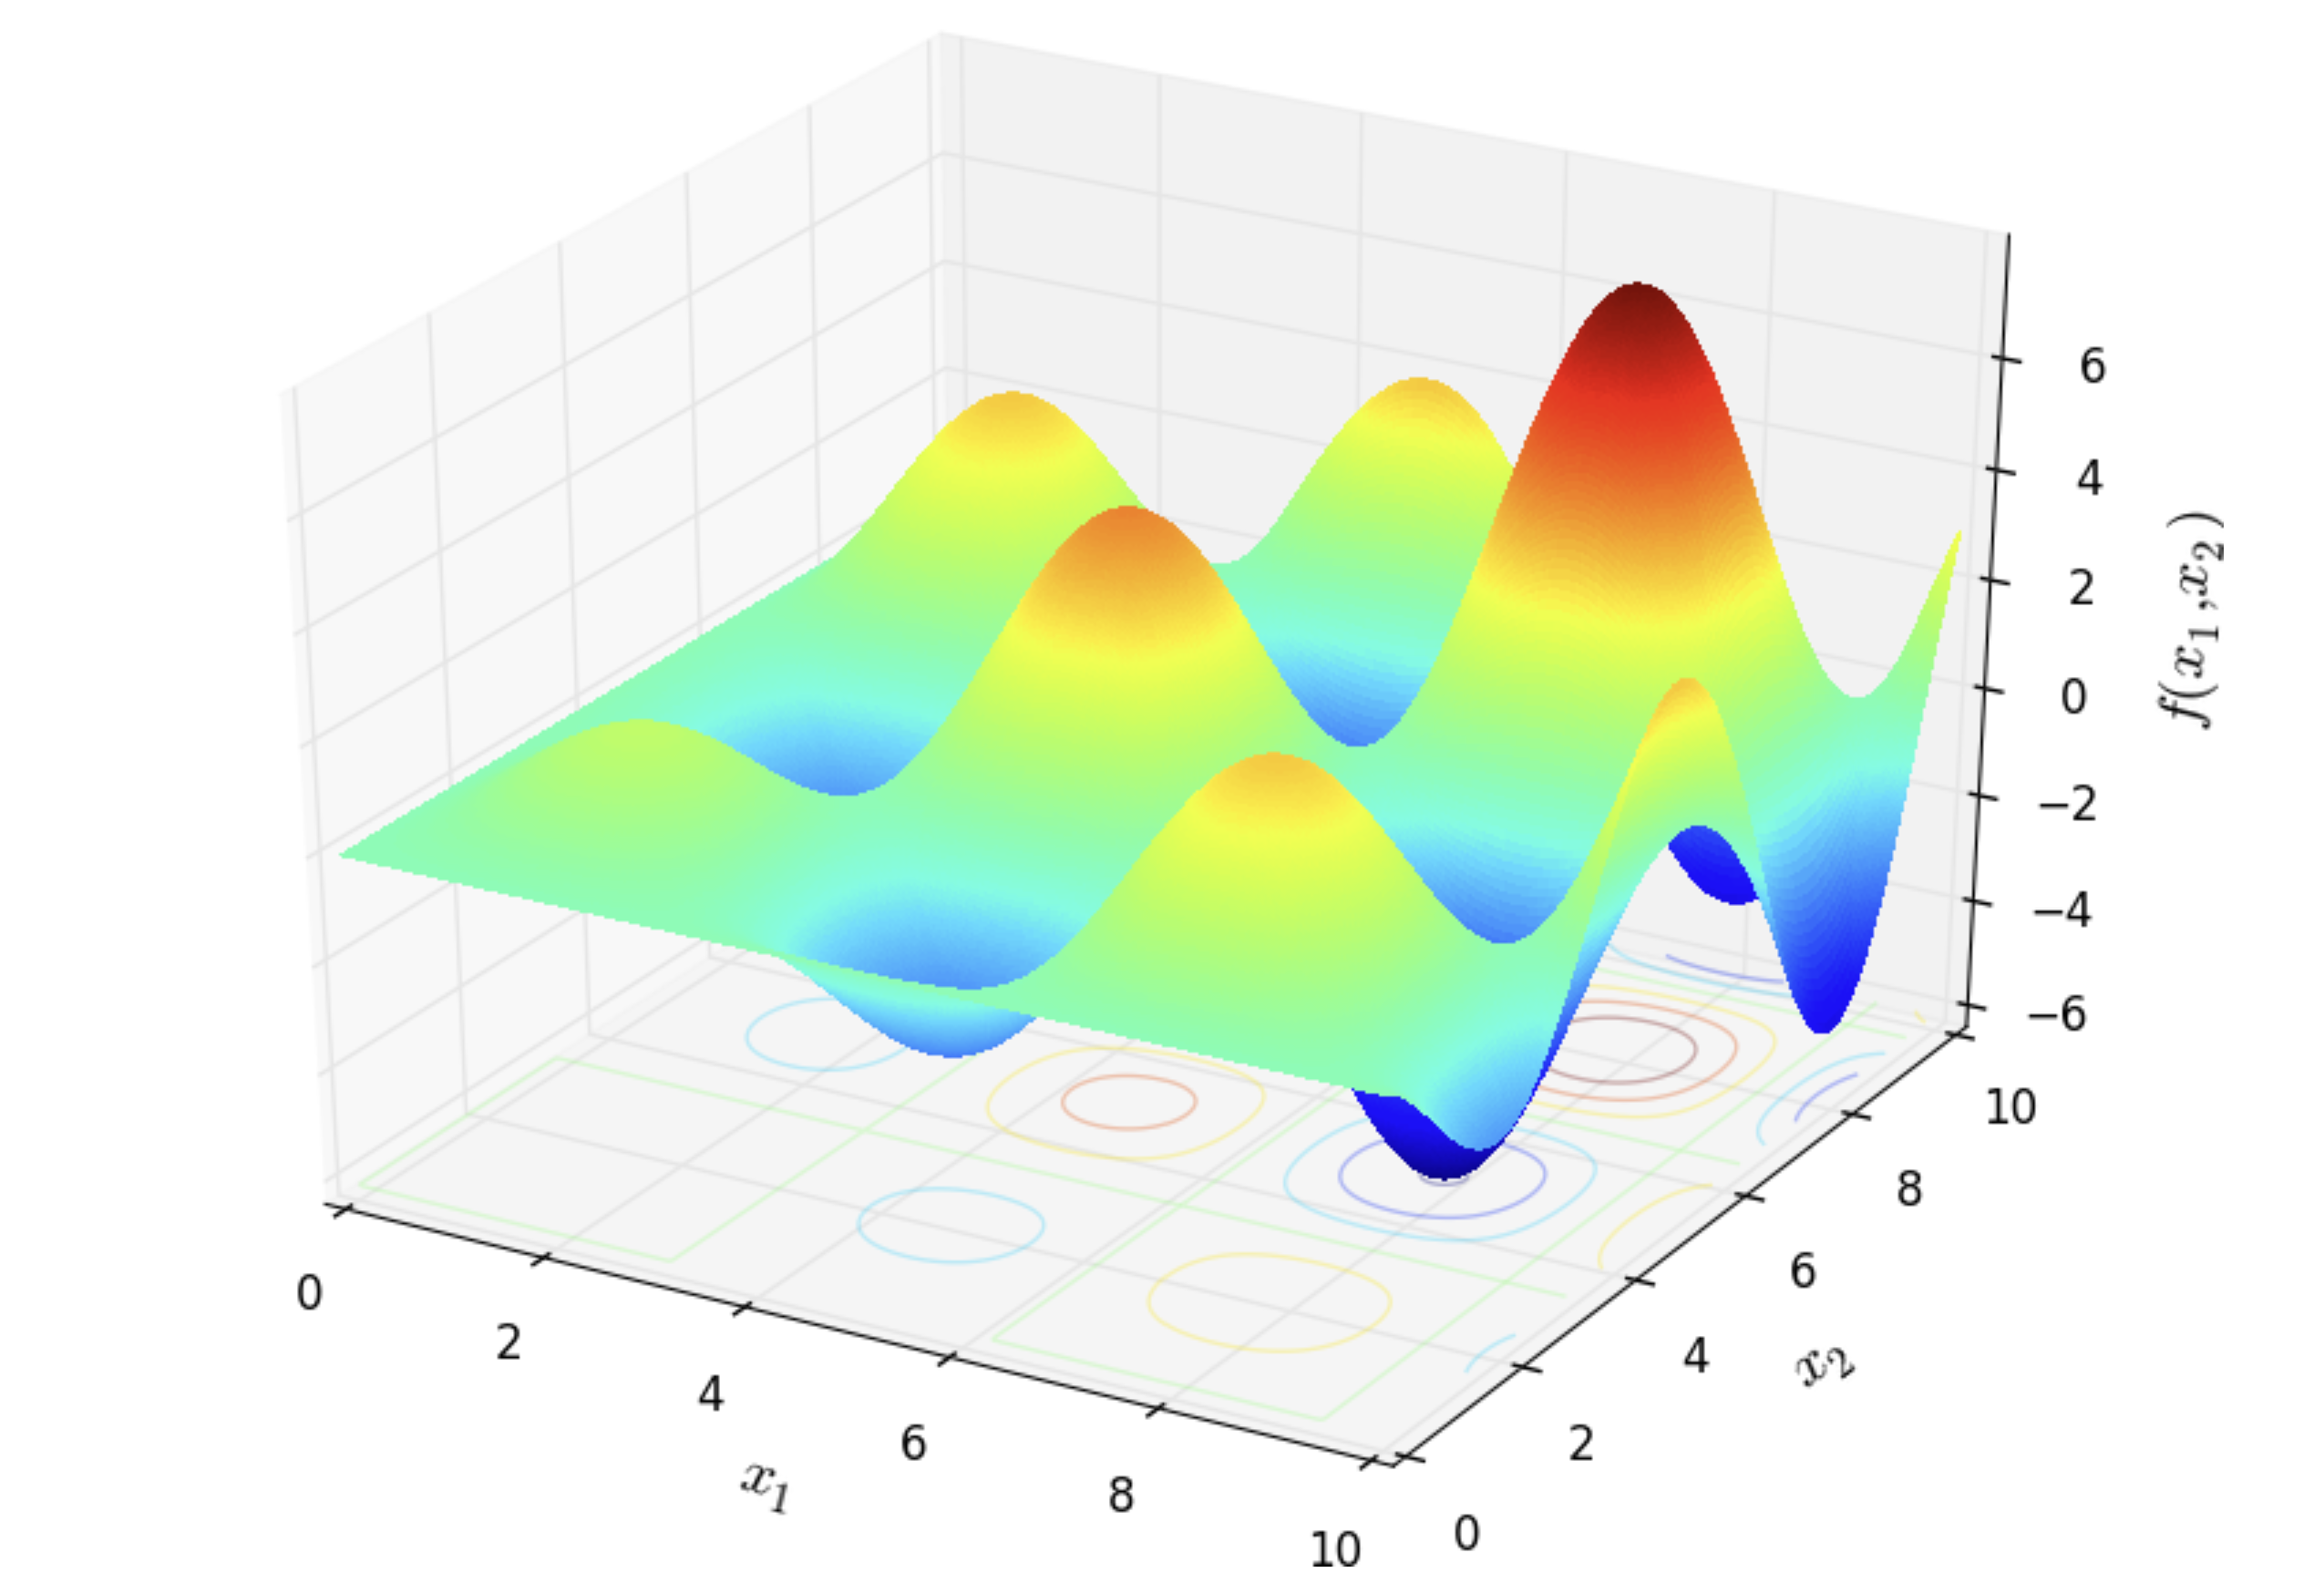
\includegraphics[scale=0.3]{images/non_convex}
			\caption{An example of non-convex function}
		\end{figure}
	\end{frame}

	\begin{frame}
		\frametitle{Tips and Tricks - Is a local minimum always a bad news?}
		
		Overfitting is around the corner. Finding a global minimum means that we have the best fit possible on the training set: this is a potentially red flag on overfitting.
		
		\vspace{5mm}
		
		Of course is better to have a convex cost function, but this is not always the case. In that cases, finding a local minimum is probably even better than a global minimum. 
		
		Remember our goal: \textbf{generalization}.
		
		\vspace{5mm}
		
		Worst case scenario: find a saddle point.
		
		
	\end{frame}
\end{document}